\chapter{الگوریتم‌های ریشه دوم}

\index{الگوریتم ریشه دوم}

یک \key{الگوریتم ریشه دوم} الگوریتمی است
که ریشه دوم در پیچیدگی زمانی آن وجود دارد.
ریشه دوم را می‌توان به عنوان «لگاریتم مرد فقیر» دید:
پیچیدگی $O(\sqrt n)$ بهتر از $O(n)$
اما بدتر از $O(\log n)$ است.
در هر حال، بسیاری از الگوریتم‌های ریشه دوم سریع و در عمل کاربردی هستند.

به عنوان مثال، مسئله ساخت یک داده‌ساختار را در نظر بگیرید
که از دو عملیات روی یک آرایه پشتیبانی می‌کند:
تغییر مقدار یک عنصر در موقعیت داده‌شده
و محاسبه مجموع عناصر در بازه داده‌شده.
پیش از این، مسئله را با استفاده از درخت‌های بازه‌ای و درخت‌های پدیدار دودویی حل کرده‌ایم
که هر دو عملیات را در زمان $O(\log n)$ پشتیبانی می‌کنند.
اما اکنون مسئله را به روش دیگری
با استفاده از یک ساختار ریشه دوم حل خواهیم کرد
که امکان تغییر عناصر در زمان $O(1)$
و محاسبه مجموع در زمان $O(\sqrt n)$ را فراهم می‌کند.

ایده کار، تقسیم آرایه به \emph{بلوک‌هایی}
به اندازه $\sqrt n$ است، به طوری که هر بلوک
شامل مجموع عناصر درون خود باشد.
به عنوان مثال، یک آرایه ۱۶ عنصری
به بلوک‌های ۴ عنصری به شکل زیر تقسیم می‌شود:

\begin{center}
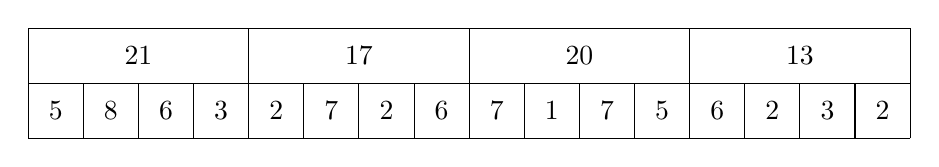
\begin{tikzpicture}[scale=0.7]
\draw (0,0) grid (16,1);

\draw (0,1) rectangle (4,2);
\draw (4,1) rectangle (8,2);
\draw (8,1) rectangle (12,2);
\draw (12,1) rectangle (16,2);

\node at (0.5, 0.5) {5};
\node at (1.5, 0.5) {8};
\node at (2.5, 0.5) {6};
\node at (3.5, 0.5) {3};
\node at (4.5, 0.5) {2};
\node at (5.5, 0.5) {7};
\node at (6.5, 0.5) {2};
\node at (7.5, 0.5) {6};
\node at (8.5, 0.5) {7};
\node at (9.5, 0.5) {1};
\node at (10.5, 0.5) {7};
\node at (11.5, 0.5) {5};
\node at (12.5, 0.5) {6};
\node at (13.5, 0.5) {2};
\node at (14.5, 0.5) {3};
\node at (15.5, 0.5) {2};

\node at (2, 1.5) {21};
\node at (6, 1.5) {17};
\node at (10, 1.5) {20};
\node at (14, 1.5) {13};

\end{tikzpicture}
\end{center}

در این ساختار،
تغییر عناصر آرایه ساده است،
زیرا پس از هر تغییر،
تنها به‌روزرسانی مجموع یک بلوک منفرد لازم است
که در زمان $O(1)$ انجام‌پذیر است.
به عنوان مثال، تصویر زیر نشان می‌دهد
که چگونه مقدار یک عنصر و مجموع بلوک متناظر آن تغییر می‌کنند:

\begin{center}
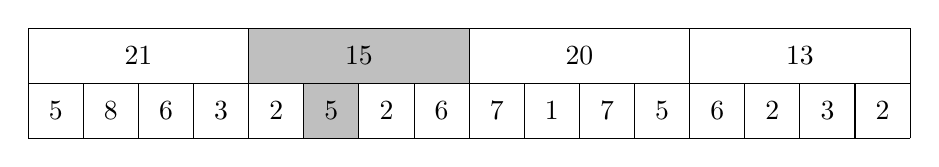
\begin{tikzpicture}[scale=0.7]
\fill[color=lightgray] (5,0) rectangle (6,1);
\draw (0,0) grid (16,1);

\fill[color=lightgray] (4,1) rectangle (8,2);
\draw (0,1) rectangle (4,2);
\draw (4,1) rectangle (8,2);
\draw (8,1) rectangle (12,2);
\draw (12,1) rectangle (16,2);

\node at (0.5, 0.5) {5};
\node at (1.5, 0.5) {8};
\node at (2.5, 0.5) {6};
\node at (3.5, 0.5) {3};
\node at (4.5, 0.5) {2};
\node at (5.5, 0.5) {5};
\node at (6.5, 0.5) {2};
\node at (7.5, 0.5) {6};
\node at (8.5, 0.5) {7};
\node at (9.5, 0.5) {1};
\node at (10.5, 0.5) {7};
\node at (11.5, 0.5) {5};
\node at (12.5, 0.5) {6};
\node at (13.5, 0.5) {2};
\node at (14.5, 0.5) {3};
\node at (15.5, 0.5) {2};

\node at (2, 1.5) {21};
\node at (6, 1.5) {15};
\node at (10, 1.5) {20};
\node at (14, 1.5) {13};

\end{tikzpicture}
\end{center}

سپس، برای محاسبه مجموع عناصر در یک بازه،
بازه را به سه بخش تقسیم می‌کنیم، به طوری که
مجموع شامل مقادیر عناصر تکی
و مجموع بلوک‌های بین آن‌ها باشد:

\begin{center}
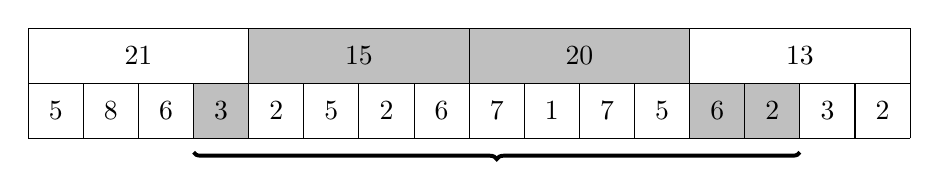
\begin{tikzpicture}[scale=0.7]
\fill[color=lightgray] (3,0) rectangle (4,1);
\fill[color=lightgray] (12,0) rectangle (13,1);
\fill[color=lightgray] (13,0) rectangle (14,1);
\draw (0,0) grid (16,1);

\fill[color=lightgray] (4,1) rectangle (8,2);
\fill[color=lightgray] (8,1) rectangle (12,2);
\draw (0,1) rectangle (4,2);
\draw (4,1) rectangle (8,2);
\draw (8,1) rectangle (12,2);
\draw (12,1) rectangle (16,2);

\node at (0.5, 0.5) {5};
\node at (1.5, 0.5) {8};
\node at (2.5, 0.5) {6};
\node at (3.5, 0.5) {3};
\node at (4.5, 0.5) {2};
\node at (5.5, 0.5) {5};
\node at (6.5, 0.5) {2};
\node at (7.5, 0.5) {6};
\node at (8.5, 0.5) {7};
\node at (9.5, 0.5) {1};
\node at (10.5, 0.5) {7};
\node at (11.5, 0.5) {5};
\node at (12.5, 0.5) {6};
\node at (13.5, 0.5) {2};
\node at (14.5, 0.5) {3};
\node at (15.5, 0.5) {2};

\node at (2, 1.5) {21};
\node at (6, 1.5) {15};
\node at (10, 1.5) {20};
\node at (14, 1.5) {13};

\draw [decoration={brace}, decorate, line width=0.5mm] (14,-0.25) -- (3,-0.25);

\end{tikzpicture}
\end{center}

از آنجا که تعداد عناصر منفرد $O(\sqrt n)$
و تعداد بلوک‌ها نیز $O(\sqrt n)$ است،
پرس‌وجوی مجموع به زمان $O(\sqrt n)$ نیاز دارد.
هدف از انتخاب اندازه بلوک $\sqrt n$ این است
که بین دو چیز \emph{تعادل} برقرار می‌کند:
آرایه به $\sqrt n$ بلوک تقسیم می‌شود،
که هر کدام شامل $\sqrt n$ عنصر است.

در عمل، نیازی نیست که از مقدار دقیق $\sqrt n$
به‌عنوان پارامتر استفاده شود،
و در عوض می‌توانیم از پارامترهای $k$ و $n/k$ بهره ببریم، جایی که $k$
متفاوت از $\sqrt n$ است.
پارامتر بهینه به مسئله و ورودی بستگی دارد.
برای مثال، اگر یک الگوریتم اغلب بلوک‌ها را پیمایش می‌کند
اما به‌ندرت عناصر منفرد درون بلوک‌ها را بررسی می‌کند،
شاید فکر خوبی باشد که آرایه را به
$k < \sqrt n$ بلوک تقسیم کنیم، که هر کدام شامل $n/k > \sqrt n$
عنصر باشد.

\section{ترکیب الگوریتم‌ها}

در این بخش دو الگوریتم جذر را بررسی می‌کنیم
که بر اساس ترکیب دو الگوریتم در یک الگوریتم پیاده‌سازی شده‌اند.
در هر دو حالت، می‌توانستیم از هر یک از الگوریتم‌ها
بدون دیگری استفاده کنیم
و مسئله را در زمان $O(n^2)$ حل کنیم.
اما با ترکیب الگوریتم‌ها، زمان اجرا
فقط $O(n \sqrt n)$ خواهد بود.

\subsubsection{پردازش حالت‌به‌حالت}

فرض کنید یک شبکه دوبعدی به ما داده شده است
که شامل $n$ خانه است.
به هر خانه یک حرف اختصاص داده شده است،
و وظیفه ما یافتن دو خانه
با حرف یکسان است که کمترین فاصله را دارند،
به‌طوری‌که فاصله میان خانه‌های
$(x_1,y_1)$ و $(x_2,y_2)$ برابر با $|x_1-x_2|+|y_1-y_2|$ باشد.
به‌عنوان مثال، شبکه زیر را در نظر بگیرید:

\begin{center}
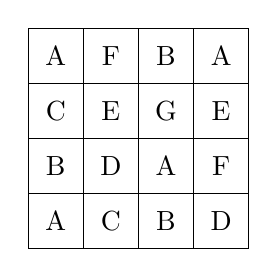
\begin{tikzpicture}[scale=0.7]
\node at (0.5,0.5) {A};
\node at (0.5,1.5) {B};
\node at (0.5,2.5) {C};
\node at (0.5,3.5) {A};
\node at (1.5,0.5) {C};
\node at (1.5,1.5) {D};
\node at (1.5,2.5) {E};
\node at (1.5,3.5) {F};
\node at (2.5,0.5) {B};
\node at (2.5,1.5) {A};
\node at (2.5,2.5) {G};
\node at (2.5,3.5) {B};
\node at (3.5,0.5) {D};
\node at (3.5,1.5) {F};
\node at (3.5,2.5) {E};
\node at (3.5,3.5) {A};
\draw (0,0) grid (4,4);
\end{tikzpicture}
\end{center}
در این حالت، کمترین فاصله برابر ۲ بین دو حرف «E» است.

می‌توان مسئله را با بررسی جداگانه هر حرف حل کرد.
با این روش، مسئله جدید محاسبه کمترین فاصله
بین دو خانه با یک حرف \emph{ثابت} $c$ است.
دو الگوریتم برای این کار بررسی می‌شود:

\emph{الگوریتم ۱:} تمام جفت‌خانه‌های دارای حرف $c$ پیمایش شده
و کمترین فاصله بین آنها محاسبه می‌شود.
زمان اجرا $O(k^2)$ است که $k$ تعداد خانه‌های دارای حرف $c$ است.

\emph{الگوریتم ۲:} یک جستجوی اول‌سطح اجرا می‌شود که همزمان
از هر خانه دارای حرف $c$ آغاز می‌گردد. کمترین فاصله بین
دو خانه با حرف $c$ در زمان $O(n)$ محاسبه خواهد شد.

یک راه، انتخاب یکی از دو الگوریتم
و استفاده از آن برای تمام حروف است.
اگر از الگوریتم ۱ استفاده شود، زمان اجرا $O(n^2)$ است،
زیرا ممکن است تمام خانه‌ها حاوی یک حرف یکسان باشند
که در این حالت $k=n$ می‌شود.
همچنین اگر از الگوریتم ۲ استفاده شود، زمان اجرا $O(n^2)$ است،
زیرا ممکن است تمام خانه‌ها حروف متفاوتی داشته باشند
و در این حالت به $n$ جستجو نیاز است.

با این حال، می‌توان دو الگوریتم را \emph{ترکیب} کرد و
بسته به تعداد دفعات تکرار هر حرف در جدول،
الگوریتم‌های متفاوتی را برای حروف مختلف به کار برد.
فرض کنید حرف $c$ به تعداد $k$ بار ظاهر شده است.
اگر $k \le \sqrt n$ باشد از الگوریتم ۱ استفاده می‌شود و اگر $k > \sqrt n$ باشد
از الگوریتم ۲ استفاده می‌گردد.
با این روش، زمان اجرای کل الگوریتم
فقط $O(n \sqrt n)$ خواهد بود.

نخست فرض کنید از الگوریتم ۱ برای حرف $c$ استفاده شود.
از آنجا که $c$ حداکثر $\sqrt n$ بار در جدول ظاهر شده،
هر خانه دارای حرف $c$ حداکثر $O(\sqrt n)$ بار
با سایر خانه‌ها مقایسه می‌شود.
بنابراین، زمان پردازش تمام این خانه‌ها $O(n \sqrt n)$ است.
سپس فرض کنید از الگوریتم ۲ برای حرف $c$ استفاده شود.
حداکثر $\sqrt n$ حرف از این نوع وجود دارد،
بنابراین پردازش این حروف نیز $O(n \sqrt n)$ زمان می‌برد.

\subsubsection{پردازش دسته‌ای}

مسئله بعدی نیز مربوط به
یک جدول دو بعدی شامل $n$ خانه است.
در ابتدا به جز یک خانه، همه خانه‌ها سفید هستند.
تعداد $n-1$ عملیات انجام می‌دهیم؛ هر عملیات ابتدا
کمترین فاصله از یک خانه سفید مشخص تا یک خانه سیاه را محاسبه کرده
و سپس آن خانه سفید را سیاه می‌کند.

به عنوان نمونه، عملیات زیر را در نظر بگیرید:

\begin{center}
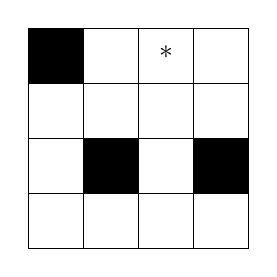
\begin{tikzpicture}[scale=0.7]
\fill[color=black] (1,1) rectangle (2,2);
\fill[color=black] (3,1) rectangle (4,2);
\fill[color=black] (0,3) rectangle (1,4);
\node at (2.5,3.5) {*};
\draw (0,0) grid (4,4);
\end{tikzpicture}
\end{center}

ابتدا کمترین فاصله را از خانه سفید مشخص‌شده با * تا یک خانه سیاه محاسبه می‌کنیم.
کمترین فاصله ۲ است، زیرا می‌توانیم با دو گام به سمت چپ به یک خانه سیاه برسیم.
سپس، خانه سفید را سیاه می‌کنیم:

\begin{center}
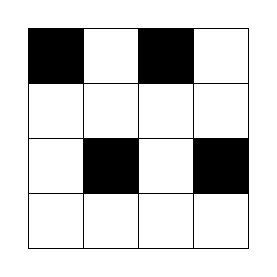
\begin{tikzpicture}[scale=0.7]
\fill[color=black] (1,1) rectangle (2,2);
\fill[color=black] (3,1) rectangle (4,2);
\fill[color=black] (0,3) rectangle (1,4);
\fill[color=black] (2,3) rectangle (3,4);
\draw (0,0) grid (4,4);
\end{tikzpicture}
\end{center}

دو الگوریتم زیر را در نظر بگیرید:

\emph{الگوریتم ۱:} استفاده از جستجوی اول‌سطح
برای محاسبه فاصله هر خانه سفید تا نزدیک‌ترین خانه سیاه.
این کار $O(n)$ زمان می‌برد و پس از جستجو،
می‌توانیم کمترین فاصله از هر خانه سفید به یک خانه سیاه را در زمان $O(1)$ پیدا کنیم.

\emph{الگوریتم ۲:} نگهداری فهرستی از خانه‌هایی که
سیاه شده‌اند، پیمایش این فهرست در هر عملیات
و سپس افزودن خانه جدید به فهرست.
یک عملیات نیازمند $O(k)$ زمان است که در آن $k$ طول فهرست است.

این دو الگوریتم را با تقسیم عملیات به
$O(\sqrt n)$ \emph{دسته} ترکیب می‌کنیم که هر کدام شامل
$O(\sqrt n)$ عملیات است.
در آغاز هر دسته،
الگوریتم ۱ را اجرا می‌کنیم.
سپس از الگوریتم ۲ برای پردازش عملیات
درون آن دسته استفاده می‌کنیم.
فهرست الگوریتم ۲ را بین دسته‌ها پاک می‌کنیم.
در هر عملیات،
کمترین فاصله تا یک خانه سیاه برابر است با کمینه فاصله محاسبه‌شده توسط الگوریتم ۱
یا فاصله محاسبه‌شده توسط الگوریتم ۲.

الگوریتم حاصل در زمان $O(n \sqrt n)$ کار می‌کند.
نخست، الگوریتم ۱ به تعداد $O(\sqrt n)$ بار اجرا می‌شود
و هر جستجو نیازمند زمان $O(n)$ است.
دوم، هنگام استفاده از الگوریتم ۲ درون یک دسته،
فهرست شامل $O(\sqrt n)$ خانه است
(زیرا فهرست بین دسته‌ها پاک می‌شود)
و هر عملیات $O(\sqrt n)$ زمان می‌برد.

\section{افرازهای عدد صحیح}

برخی از الگوریتم‌های ریشه دوم بر این مشاهده استوارند:
اگر یک عدد صحیح مثبت $n$ به صورت مجموعی از اعداد صحیح مثبت نمایش داده شود،
چنین مجموعی همواره حداکثر شامل $O(\sqrt n)$ عدد \emph{متمایز} است.
دلیل این است که برای ساختن مجموعی با بیشترین تعداد اعداد متمایز،
باید اعداد \emph{کوچک} را برگزینیم.
اگر اعداد $1,2,\ldots,k$ را انتخاب کنیم،
مجموع حاصل برابر است با:
\[\frac{k(k+1)}{2}.\]
بنابراین، حداکثر تعداد اعداد متمایز برابر است با $k = O(\sqrt n)$.
در ادامه دو مسئله را بررسی می‌کنیم که با استفاده از این مشاهده به صورت کارا حل می‌شوند.

\subsubsection{کوله‌پشتی}

فرض کنید فهرستی از وزن‌های صحیح با مجموع $n$ داده شده است.
مسئله پیدا کردن تمام مجموع‌هایی است که می‌توان با زیرمجموعه‌ای از این وزن‌ها ساخت. برای نمونه، اگر وزن‌ها $\{1,3,3\}$ باشند، مجموع‌های ممکن به شرح زیر هستند:

\begin{itemize}[noitemsep]
\item $0$ (مجموعه تهی)
\item $1$
\item $3$
\item $1+3=4$
\item $3+3=6$
\item $1+3+3=7$
\end{itemize}

با استفاده از روش کوله‌پشتی استاندارد (بخش ۷.۴ را ببینید)،
مسئله را می‌توان به این صورت حل کرد:
تابع $\texttt{possible}(x,k)$ را تعریف می‌کنیم که مقدار آن برابر ۱ است
اگر بتوان مجموع $x$ را با استفاده از $k$ وزن اول ساخت،
و در غیر این صورت ۰ است.
از آنجا که مجموع وزن‌ها برابر $n$ است،
حداکثر $n$ وزن وجود دارد و
تمام مقادیر این تابع را می‌توان
در زمان $O(n^2)$ با استفاده از برنامه‌نویسی پویا محاسبه کرد.

با این حال، می‌توان الگوریتم را کارآمدتر کرد
با استفاده از این واقعیت که حداکثر $O(\sqrt n)$
وزن \emph{متمایز} وجود دارد.
بنابراین، می‌توانیم وزن‌ها را در گروه‌هایی پردازش کنیم
که شامل وزن‌های یکسان هستند.
هر گروه را می‌توان
در زمان $O(n)$ پردازش کرد، که الگوریتمی با زمان اجرای $O(n \sqrt n)$ به دست می‌دهد.

ایده این است که از آرایه‌ای استفاده کنیم که مجموع وزن‌های قابل ساخت
با استفاده از گروه‌های پردازش‌شده تاکنون را ثبت کند.
این آرایه شامل $n$ عنصر است: عنصر $k$ برابر ۱ است اگر مجموع
$k$ قابل ساخت باشد و در غیر این صورت ۰ است.
برای پردازش یک گروه از وزن‌ها، آرایه را
از چپ به راست پیمایش می‌کنیم و مجموع‌های جدیدی را که
می‌توان با استفاده از این گروه و گروه‌های قبلی ساخت، ثبت می‌نماییم.

\subsubsection{ساخت رشته}

به ازای رشته \texttt{s} به طول $n$
و مجموعه‌ای از رشته‌ها $D$ با مجموع طول $m$،
مسئله شمارش تعداد روش‌های ساخت
\texttt{s} به صورت الحاق رشته‌های موجود در $D$ را در نظر بگیرید.
به عنوان مثال،
اگر $\texttt{s}=\texttt{ABAB}$ و
$D=\{\texttt{A},\texttt{B},\texttt{AB}\}$ باشد،
۴ روش وجود دارد:

\begin{itemize}[noitemsep]
\item $\texttt{A}+\texttt{B}+\texttt{A}+\texttt{B}$
\item $\texttt{AB}+\texttt{A}+\texttt{B}$
\item $\texttt{A}+\texttt{B}+\texttt{AB}$
\item $\texttt{AB}+\texttt{AB}$
\end{itemize}

می‌توان مسئله را با استفاده از برنامه‌نویسی پویا حل کرد:
فرض کنید $\texttt{count}(k)$ نشان‌دهنده تعداد روش‌های ساخت پیشوند
$\texttt{s}[0 \ldots k]$ با استفاده از رشته‌های موجود در $D$ باشد.
اکنون $\texttt{count}(n-1)$ پاسخ مسئله را می‌دهد،
و می‌توان مسئله را در زمان $O(n^2)$
با استفاده از ساختمان داده ترای (trie) حل کرد.

با این حال، می‌توان مسئله را به شکل کارآمدتری حل کرد
با استفاده از هشینگ رشته و این واقعیت که
حداکثر $O(\sqrt m)$ طول متمایز برای رشته‌ها در $D$ وجود دارد.
ابتدا، مجموعه $H$ را می‌سازیم که شامل مقادیر هش
تمام رشته‌های موجود در $D$ است.
سپس، هنگام محاسبه مقدار $\texttt{count}(k)$،
تمام مقادیر $p$ را بررسی می‌کنیم
به طوری که رشته‌ای با طول $p$ در $D$ وجود داشته باشد،
مقدار هش $\texttt{s}[k-p+1 \ldots k]$ را محاسبه کرده
و بررسی می‌کنیم که آیا متعلق به $H$ است یا خیر.
از آنجا که حداکثر $O(\sqrt m)$ طول رشته متمایز وجود دارد،
این کار منجر به الگوریتمی با زمان اجرای $O(n \sqrt m)$ می‌شود.

\section{الگوریتم مو (Mo's algorithm)}

\index{Mo's algorithm}

\key{الگوریتم مو}\footnote{بر اساس \cite{cod15}، این الگوریتم به نام مو تائو (Mo Tao)، یک برنامه‌نویس رقابتی اهل چین، نام‌گذاری شده است، اما این روش پیش‌تر نیز در مقالات علمی مطرح شده بود \cite{ken06}.}
می‌تواند در مسائل متعددی به کار رود که نیازمند پردازش پرسش‌های بازه‌ای روی یک آرایه \emph{ایستا} هستند؛ یعنی مقادیر آرایه بین پرسش‌ها تغییر نمی‌کنند.
در هر پرسش، یک بازه $[a,b]$ داده می‌شود و باید مقداری را بر اساس عناصر آرایه بین موقعیت‌های $a$ و $b$ محاسبه کنیم.
از آنجا که آرایه ایستا است، پرسش‌ها را می‌توان به هر ترتیبی پردازش کرد.
الگوریتم مو پرسش‌ها را با ترتیب ویژه‌ای پردازش می‌کند که اجرای کارآمد الگوریتم را تضمین می‌نماید.

الگوریتم مو یک \emph{بازه فعال} از آرایه را نگهداری می‌کند و پاسخ پرسش مربوط به بازه فعال در هر لحظه مشخص است.
الگوریتم پرسش‌ها را یکی پس از دیگری پردازش می‌کند و همیشه با افزودن و حذف عناصر، نقاط انتهایی بازه فعال را جابجا می‌کند.
پیچیدگی زمانی الگوریتم $O(n \sqrt n f(n))$ است که در آن آرایه شامل $n$ عنصر است، $n$ پرسش وجود دارد و هر درج و حذف یک عنصر نیازمند زمان $O(f(n))$ است.

ترفند الگوریتم مو در ترتیب پردازش پرسش‌ها نهفته است:
آرایه به بلوک‌هایی شامل $k=O(\sqrt n)$ عنصر تقسیم می‌شود، و پرسش $[a_1,b_1]$ قبل از پرسش $[a_2,b_2]$ پردازش می‌شود اگر:
\begin{itemize}
\item $\lfloor a_1/k \rfloor < \lfloor a_2/k \rfloor$ یا
\item $\lfloor a_1/k \rfloor = \lfloor a_2/k \rfloor$ و $b_1 < b_2$.
\end{itemize}

بدین ترتیب، تمام پرسش‌هایی که نقطه انتهایی چپ آن‌ها در یک بلوک مشخص قرار دارد، پشت سر هم و بر اساس نقطه انتهایی راست مرتب و پردازش می‌شوند.
با استفاده از این ترتیب، الگوریتم تنها $O(n \sqrt n)$ عملیات انجام می‌دهد، زیرا نقطه انتهایی چپ $O(n)$ بار و هر بار $O(\sqrt n)$ گام جابجا می‌شود، و نقطه انتهایی راست $O(\sqrt n)$ بار و هر بار $O(n)$ گام جابجا می‌شود. بنابراین، هر دو نقطه انتهایی در طول اجرای الگوریتم مجموعاً $O(n \sqrt n)$ گام جابجا می‌شوند.

\subsubsection*{مثال}

به عنوان مثال، مسئله‌ای را در نظر بگیرید که در آن مجموعه‌ای از پرسش‌ها داده شده است، هر پرسش مربوط به بازه‌ای در یک آرایه است، و وظیفه ما محاسبه تعداد عناصر \emph{متمایز} در آن بازه برای هر پرسش است.

در الگوریتم مو، پرسش‌ها همواره به یک شکل مرتب می‌شوند، اما نحوه نگهداری پاسخ پرسش به نوع مسئله بستگی دارد.
در این مسئله، می‌توانیم یک آرایه \texttt{count} نگه داریم که در آن $\texttt{count}[x]$ نشان‌دهنده تعداد دفعات تکرار عنصر $x$ در بازه فعال است.

وقتی از پرس‌وجویی به پرس‌وجوی دیگر می‌رویم،
بازه فعال تغییر می‌کند.
برای نمونه، اگر بازه کنونی
\begin{center}
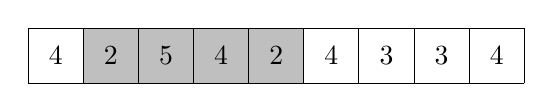
\begin{tikzpicture}[scale=0.7]
\fill[color=lightgray] (1,0) rectangle (5,1);
\draw (0,0) grid (9,1);
\node at (0.5, 0.5) {4};
\node at (1.5, 0.5) {2};
\node at (2.5, 0.5) {5};
\node at (3.5, 0.5) {4};
\node at (4.5, 0.5) {2};
\node at (5.5, 0.5) {4};
\node at (6.5, 0.5) {3};
\node at (7.5, 0.5) {3};
\node at (8.5, 0.5) {4};
\end{tikzpicture}
\end{center}
و بازه بعدی
\begin{center}
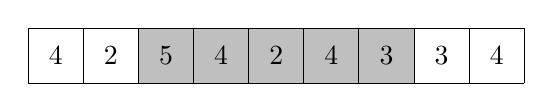
\begin{tikzpicture}[scale=0.7]
\fill[color=lightgray] (2,0) rectangle (7,1);
\draw (0,0) grid (9,1);
\node at (0.5, 0.5) {4};
\node at (1.5, 0.5) {2};
\node at (2.5, 0.5) {5};
\node at (3.5, 0.5) {4};
\node at (4.5, 0.5) {2};
\node at (5.5, 0.5) {4};
\node at (6.5, 0.5) {3};
\node at (7.5, 0.5) {3};
\node at (8.5, 0.5) {4};
\end{tikzpicture}
\end{center}
باشد، سه گام خواهیم داشت:
نقطه پایانی چپ یک گام به راست می‌رود،
و نقطه پایانی راست دو گام به راست می‌رود.

پس از هر گام، آرایه \texttt{count}
باید به‌روزرسانی شود.
پس از افزودن عنصر $x$،
مقدار $\texttt{count}[x]$ را یک واحد افزایش می‌دهیم،
و اگر پس از این کار $\texttt{count}[x]=1$ شد،
پاسخ پرس‌وجو را نیز یک واحد افزایش می‌دهیم.
به‌طور مشابه، پس از حذف عنصر $x$،
مقدار $\texttt{count}[x]$ را یک واحد کاهش می‌دهیم،
و اگر پس از این کار $\texttt{count}[x]=0$ شد،
پاسخ پرس‌وجو را نیز یک واحد کاهش می‌دهیم.

در این مسئله، زمان مورد نیاز برای اجرای
هر گام $O(1)$ است، بنابراین پیچیدگی زمانی کل
الگوریتم $O(n \sqrt n)$ است.